\chapter{Aufbau und Systemarchitektur}

\section{Systemarchitektur – Web-Applikation}

\section*{Erklärung}
Die Systemarchitektur der Webanwendung besteht grundsätzlich aus zwei Teilen. Dem auf NGINX [\ref{sec:NGINX}] basierenden Server und dem Client der per Browser die Seite aufruft. Auf dem Server sind alle benötigten Dateien und die Logik. In den Dateien, die in JavaScript geschrieben wurden, befinden sich die Modelle, die Animationen und die Geschäftslogik. Diese werden dann an den Browser übermittelt und gerendert.

\section*{Deployment}
Um die Aufwendung auf einem Server zu deployen und um sie anschließend zu verwenden, müssen einige Kriterien erfüllt werden. Es muss ein NGINX-Server [\ref{sec:NGINX}] vorliegen auf dem die index.html und die JavaScript Dateien hochgeladen wurden. Erst diese ermöglichen den Start der Anwendung, zusätzliche Schritte sind nicht von Nöten.

\begin{figure}
    \centering
    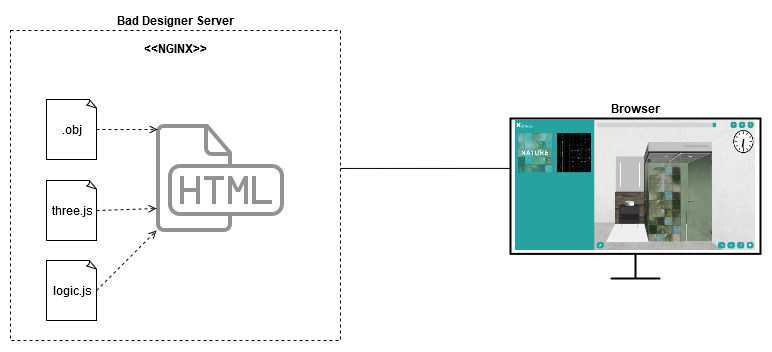
\includegraphics[scale=.4]{images/DA-SysArch.jpg}
    \caption{Systemarchitektur der Web-Applikation}
\end{figure}


\section{Systemarchitektur – Electron Anwendung}

\section*{Erklärung}
Das Electron Executable muss lediglich vom Server heruntergeladen werden und installiert werden. Danach ist die Anwendung sofort einsetzbar. Dadurch das die Applikation mit Electron \ref{sec:Electron} gemacht wurde lässt sie sich wie eine normale Desktopanwendung starten ohne Browser.

\section*{Deployment}
Um die Diplomarbeit als Electron Anwendung zu deployen und benützen muss man lediglich die bestehende Web-App in eine Electron App konvertieren und auf dem Server zum Herunterladen stellen.
